\documentclass[twoside]{book}

% Packages required by doxygen
\usepackage{calc}
\usepackage{doxygen}
\usepackage{graphicx}
\usepackage[utf8]{inputenc}
\usepackage{makeidx}
\usepackage{multicol}
\usepackage{multirow}
\usepackage{textcomp}
\usepackage[table]{xcolor}

% Font selection
\usepackage[T1]{fontenc}
\usepackage{mathptmx}
\usepackage[scaled=.90]{helvet}
\usepackage{courier}
\usepackage{amssymb}
\usepackage{sectsty}
\renewcommand{\familydefault}{\sfdefault}
\allsectionsfont{%
  \fontseries{bc}\selectfont%
  \color{darkgray}%
}
\renewcommand{\DoxyLabelFont}{%
  \fontseries{bc}\selectfont%
  \color{darkgray}%
}

% Page & text layout
\usepackage{geometry}
\geometry{%
  a4paper,%
  top=2.5cm,%
  bottom=2.5cm,%
  left=2.5cm,%
  right=2.5cm%
}
\tolerance=750
\hfuzz=15pt
\hbadness=750
\setlength{\emergencystretch}{15pt}
\setlength{\parindent}{0cm}
\setlength{\parskip}{0.2cm}
\makeatletter
\renewcommand{\paragraph}{%
  \@startsection{paragraph}{4}{0ex}{-1.0ex}{1.0ex}{%
    \normalfont\normalsize\bfseries\SS@parafont%
  }%
}
\renewcommand{\subparagraph}{%
  \@startsection{subparagraph}{5}{0ex}{-1.0ex}{1.0ex}{%
    \normalfont\normalsize\bfseries\SS@subparafont%
  }%
}
\makeatother

% Headers & footers
\usepackage{fancyhdr}
\pagestyle{fancyplain}
\fancyhead[LE]{\fancyplain{}{\bfseries\thepage}}
\fancyhead[CE]{\fancyplain{}{}}
\fancyhead[RE]{\fancyplain{}{\bfseries\leftmark}}
\fancyhead[LO]{\fancyplain{}{\bfseries\rightmark}}
\fancyhead[CO]{\fancyplain{}{}}
\fancyhead[RO]{\fancyplain{}{\bfseries\thepage}}
\fancyfoot[LE]{\fancyplain{}{}}
\fancyfoot[CE]{\fancyplain{}{}}
\fancyfoot[RE]{\fancyplain{}{\bfseries\scriptsize Generated on Sun Apr 24 2016 21\-:41\-:01 for Message\-Ticker by Doxygen }}
\fancyfoot[LO]{\fancyplain{}{\bfseries\scriptsize Generated on Sun Apr 24 2016 21\-:41\-:01 for Message\-Ticker by Doxygen }}
\fancyfoot[CO]{\fancyplain{}{}}
\fancyfoot[RO]{\fancyplain{}{}}
\renewcommand{\footrulewidth}{0.4pt}
\renewcommand{\chaptermark}[1]{%
  \markboth{#1}{}%
}
\renewcommand{\sectionmark}[1]{%
  \markright{\thesection\ #1}%
}

% Indices & bibliography
\usepackage{natbib}
\usepackage[titles]{tocloft}
\setcounter{tocdepth}{3}
\setcounter{secnumdepth}{5}
\makeindex

% Hyperlinks (required, but should be loaded last)
\usepackage{ifpdf}
\ifpdf
  \usepackage[pdftex,pagebackref=true]{hyperref}
\else
  \usepackage[ps2pdf,pagebackref=true]{hyperref}
\fi
\hypersetup{%
  colorlinks=true,%
  linkcolor=blue,%
  citecolor=blue,%
  unicode%
}

% Custom commands
\newcommand{\clearemptydoublepage}{%
  \newpage{\pagestyle{empty}\cleardoublepage}%
}


%===== C O N T E N T S =====

\begin{document}

% Titlepage & ToC
\hypersetup{pageanchor=false}
\pagenumbering{roman}
\begin{titlepage}
\vspace*{7cm}
\begin{center}%
{\Large Message\-Ticker \\[1ex]\large 1.\-0 }\\
\vspace*{1cm}
{\large Generated by Doxygen 1.8.6}\\
\vspace*{0.5cm}
{\small Sun Apr 24 2016 21:41:01}\\
\end{center}
\end{titlepage}
\clearemptydoublepage
\tableofcontents
\clearemptydoublepage
\pagenumbering{arabic}
\hypersetup{pageanchor=true}

%--- Begin generated contents ---
\chapter{Hierarchical Index}
\section{Class Hierarchy}
This inheritance list is sorted roughly, but not completely, alphabetically\-:\begin{DoxyCompactList}
\item J\-Frame\begin{DoxyCompactList}
\item \contentsline{section}{de.\-haw.\-rnp.\-messageticker.\-view.\-Messages\-View}{\pageref{classde_1_1haw_1_1rnp_1_1messageticker_1_1view_1_1MessagesView}}{}
\end{DoxyCompactList}
\item \contentsline{section}{de.\-haw.\-rnp.\-messageticker.\-Main}{\pageref{classde_1_1haw_1_1rnp_1_1messageticker_1_1Main}}{}
\item \contentsline{section}{de.\-haw.\-rnp.\-messageticker.\-model.\-Message}{\pageref{classde_1_1haw_1_1rnp_1_1messageticker_1_1model_1_1Message}}{}
\item \contentsline{section}{de.\-haw.\-rnp.\-messageticker.\-model.\-Message\-Test}{\pageref{classde_1_1haw_1_1rnp_1_1messageticker_1_1model_1_1MessageTest}}{}
\item \contentsline{section}{de.\-haw.\-rnp.\-messageticker.\-model.\-Random\-Generator}{\pageref{classde_1_1haw_1_1rnp_1_1messageticker_1_1model_1_1RandomGenerator}}{}
\item \contentsline{section}{de.\-haw.\-rnp.\-messageticker.\-model.\-Random\-Generator\-Test}{\pageref{classde_1_1haw_1_1rnp_1_1messageticker_1_1model_1_1RandomGeneratorTest}}{}
\item Runnable\begin{DoxyCompactList}
\item \contentsline{section}{de.\-haw.\-rnp.\-messageticker.\-Controller}{\pageref{classde_1_1haw_1_1rnp_1_1messageticker_1_1Controller}}{}
\end{DoxyCompactList}
\item Thread\begin{DoxyCompactList}
\item \contentsline{section}{de.\-haw.\-rnp.\-messageticker.\-model.\-Message\-Producer}{\pageref{classde_1_1haw_1_1rnp_1_1messageticker_1_1model_1_1MessageProducer}}{}
\end{DoxyCompactList}
\item Action\-Listener\begin{DoxyCompactList}
\item \contentsline{section}{de.\-haw.\-rnp.\-messageticker.\-model.\-General\-Purpose\-Listener}{\pageref{classde_1_1haw_1_1rnp_1_1messageticker_1_1model_1_1GeneralPurposeListener}}{}
\end{DoxyCompactList}
\end{DoxyCompactList}

\chapter{Class Index}
\section{Class List}
Here are the classes, structs, unions and interfaces with brief descriptions\-:\begin{DoxyCompactList}
\item\contentsline{section}{\hyperlink{classde_1_1haw_1_1rnp_1_1messageticker_1_1Controller}{de.\-haw.\-rnp.\-messageticker.\-Controller} \\*\hyperlink{classde_1_1haw_1_1rnp_1_1messageticker_1_1Controller}{Controller} for the M\-V\-C Pattern }{\pageref{classde_1_1haw_1_1rnp_1_1messageticker_1_1Controller}}{}
\item\contentsline{section}{\hyperlink{classde_1_1haw_1_1rnp_1_1messageticker_1_1model_1_1GeneralPurposeListener}{de.\-haw.\-rnp.\-messageticker.\-model.\-General\-Purpose\-Listener} \\*Listener that just forwards the actions back to the controller (for better modularity) }{\pageref{classde_1_1haw_1_1rnp_1_1messageticker_1_1model_1_1GeneralPurposeListener}}{}
\item\contentsline{section}{\hyperlink{classde_1_1haw_1_1rnp_1_1messageticker_1_1Main}{de.\-haw.\-rnp.\-messageticker.\-Main} }{\pageref{classde_1_1haw_1_1rnp_1_1messageticker_1_1Main}}{}
\item\contentsline{section}{\hyperlink{classde_1_1haw_1_1rnp_1_1messageticker_1_1model_1_1Message}{de.\-haw.\-rnp.\-messageticker.\-model.\-Message} \\*This class represents a message }{\pageref{classde_1_1haw_1_1rnp_1_1messageticker_1_1model_1_1Message}}{}
\item\contentsline{section}{\hyperlink{classde_1_1haw_1_1rnp_1_1messageticker_1_1model_1_1MessageProducer}{de.\-haw.\-rnp.\-messageticker.\-model.\-Message\-Producer} \\*Producer in the consumer producer pattern }{\pageref{classde_1_1haw_1_1rnp_1_1messageticker_1_1model_1_1MessageProducer}}{}
\item\contentsline{section}{\hyperlink{classde_1_1haw_1_1rnp_1_1messageticker_1_1view_1_1MessagesView}{de.\-haw.\-rnp.\-messageticker.\-view.\-Messages\-View} \\*The view for displaying all messages and the basic chat functionality }{\pageref{classde_1_1haw_1_1rnp_1_1messageticker_1_1view_1_1MessagesView}}{}
\item\contentsline{section}{\hyperlink{classde_1_1haw_1_1rnp_1_1messageticker_1_1model_1_1MessageTest}{de.\-haw.\-rnp.\-messageticker.\-model.\-Message\-Test} \\*Tests for the \hyperlink{classde_1_1haw_1_1rnp_1_1messageticker_1_1model_1_1Message}{Message} Model }{\pageref{classde_1_1haw_1_1rnp_1_1messageticker_1_1model_1_1MessageTest}}{}
\item\contentsline{section}{\hyperlink{classde_1_1haw_1_1rnp_1_1messageticker_1_1model_1_1RandomGenerator}{de.\-haw.\-rnp.\-messageticker.\-model.\-Random\-Generator} \\*Generator for random messages and other stuff with the singleton pattern }{\pageref{classde_1_1haw_1_1rnp_1_1messageticker_1_1model_1_1RandomGenerator}}{}
\item\contentsline{section}{\hyperlink{classde_1_1haw_1_1rnp_1_1messageticker_1_1model_1_1RandomGeneratorTest}{de.\-haw.\-rnp.\-messageticker.\-model.\-Random\-Generator\-Test} \\*Tests the \hyperlink{classde_1_1haw_1_1rnp_1_1messageticker_1_1model_1_1RandomGenerator}{Random\-Generator} }{\pageref{classde_1_1haw_1_1rnp_1_1messageticker_1_1model_1_1RandomGeneratorTest}}{}
\end{DoxyCompactList}

\chapter{Class Documentation}
\hypertarget{classde_1_1haw_1_1rnp_1_1messageticker_1_1Controller}{\section{de.\-haw.\-rnp.\-messageticker.\-Controller Class Reference}
\label{classde_1_1haw_1_1rnp_1_1messageticker_1_1Controller}\index{de.\-haw.\-rnp.\-messageticker.\-Controller@{de.\-haw.\-rnp.\-messageticker.\-Controller}}
}


\hyperlink{classde_1_1haw_1_1rnp_1_1messageticker_1_1Controller}{Controller} for the M\-V\-C Pattern.  


Inheritance diagram for de.\-haw.\-rnp.\-messageticker.\-Controller\-:\begin{figure}[H]
\begin{center}
\leavevmode
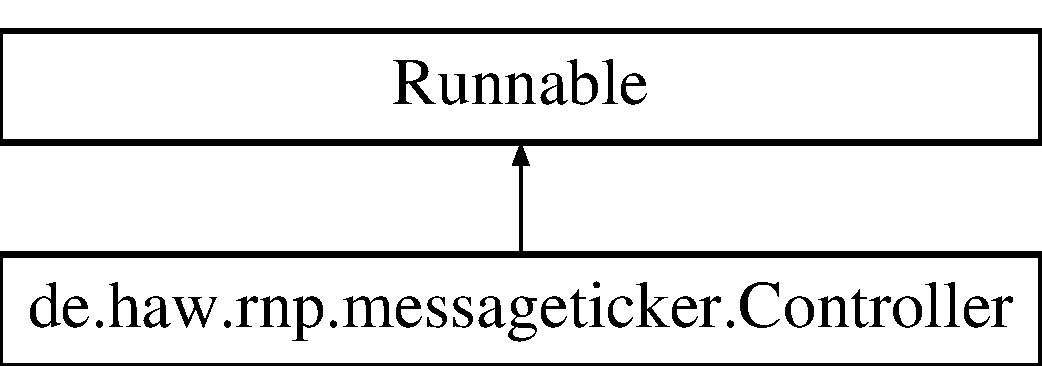
\includegraphics[height=2.000000cm]{classde_1_1haw_1_1rnp_1_1messageticker_1_1Controller}
\end{center}
\end{figure}
\subsection*{Public Member Functions}
\begin{DoxyCompactItemize}
\item 
\hyperlink{classde_1_1haw_1_1rnp_1_1messageticker_1_1Controller_ac8e9fae5cb88bfce79183a0083461c83}{Controller} (int thread\-Count)
\begin{DoxyCompactList}\small\item\em Constructs the \hyperlink{classde_1_1haw_1_1rnp_1_1messageticker_1_1Controller}{Controller} with a thread pool. \end{DoxyCompactList}\item 
\hypertarget{classde_1_1haw_1_1rnp_1_1messageticker_1_1Controller_af8a2b3982f049feff0033438cb7e903f}{void {\bfseries show\-View} ()}\label{classde_1_1haw_1_1rnp_1_1messageticker_1_1Controller_af8a2b3982f049feff0033438cb7e903f}

\item 
\hypertarget{classde_1_1haw_1_1rnp_1_1messageticker_1_1Controller_a9af1c749b25a86bccd8ca1082bd1e164}{void {\bfseries run} ()}\label{classde_1_1haw_1_1rnp_1_1messageticker_1_1Controller_a9af1c749b25a86bccd8ca1082bd1e164}

\item 
void \hyperlink{classde_1_1haw_1_1rnp_1_1messageticker_1_1Controller_a3d64a8b1ca98d53d3ee7f8b4585dd306}{perform\-Action} (Action\-Event e)
\begin{DoxyCompactList}\small\item\em Handles the actions from the General\-Purpose\-Listener. \end{DoxyCompactList}\end{DoxyCompactItemize}


\subsection{Detailed Description}
\hyperlink{classde_1_1haw_1_1rnp_1_1messageticker_1_1Controller}{Controller} for the M\-V\-C Pattern. 

\subsection{Constructor \& Destructor Documentation}
\hypertarget{classde_1_1haw_1_1rnp_1_1messageticker_1_1Controller_ac8e9fae5cb88bfce79183a0083461c83}{\index{de\-::haw\-::rnp\-::messageticker\-::\-Controller@{de\-::haw\-::rnp\-::messageticker\-::\-Controller}!Controller@{Controller}}
\index{Controller@{Controller}!de::haw::rnp::messageticker::Controller@{de\-::haw\-::rnp\-::messageticker\-::\-Controller}}
\subsubsection[{Controller}]{\setlength{\rightskip}{0pt plus 5cm}de.\-haw.\-rnp.\-messageticker.\-Controller.\-Controller (
\begin{DoxyParamCaption}
\item[{int}]{thread\-Count}
\end{DoxyParamCaption}
)}}\label{classde_1_1haw_1_1rnp_1_1messageticker_1_1Controller_ac8e9fae5cb88bfce79183a0083461c83}


Constructs the \hyperlink{classde_1_1haw_1_1rnp_1_1messageticker_1_1Controller}{Controller} with a thread pool. 


\begin{DoxyParams}{Parameters}
{\em thread\-Count} & count of the threads in the pool \\
\hline
\end{DoxyParams}


\subsection{Member Function Documentation}
\hypertarget{classde_1_1haw_1_1rnp_1_1messageticker_1_1Controller_a3d64a8b1ca98d53d3ee7f8b4585dd306}{\index{de\-::haw\-::rnp\-::messageticker\-::\-Controller@{de\-::haw\-::rnp\-::messageticker\-::\-Controller}!perform\-Action@{perform\-Action}}
\index{perform\-Action@{perform\-Action}!de::haw::rnp::messageticker::Controller@{de\-::haw\-::rnp\-::messageticker\-::\-Controller}}
\subsubsection[{perform\-Action}]{\setlength{\rightskip}{0pt plus 5cm}void de.\-haw.\-rnp.\-messageticker.\-Controller.\-perform\-Action (
\begin{DoxyParamCaption}
\item[{Action\-Event}]{e}
\end{DoxyParamCaption}
)}}\label{classde_1_1haw_1_1rnp_1_1messageticker_1_1Controller_a3d64a8b1ca98d53d3ee7f8b4585dd306}


Handles the actions from the General\-Purpose\-Listener. 


\begin{DoxyParams}{Parameters}
{\em e} & Action\-Event \\
\hline
\end{DoxyParams}
Adds the message from the View into the queue

Stops and restarts all threads

The documentation for this class was generated from the following file\-:\begin{DoxyCompactItemize}
\item 
src/main/java/de/haw/rnp/messageticker/Controller.\-java\end{DoxyCompactItemize}

\hypertarget{classde_1_1haw_1_1rnp_1_1messageticker_1_1model_1_1GeneralPurposeListener}{\section{de.\-haw.\-rnp.\-messageticker.\-model.\-General\-Purpose\-Listener Class Reference}
\label{classde_1_1haw_1_1rnp_1_1messageticker_1_1model_1_1GeneralPurposeListener}\index{de.\-haw.\-rnp.\-messageticker.\-model.\-General\-Purpose\-Listener@{de.\-haw.\-rnp.\-messageticker.\-model.\-General\-Purpose\-Listener}}
}


Listener that just forwards the actions back to the controller (for better modularity).  


Inheritance diagram for de.\-haw.\-rnp.\-messageticker.\-model.\-General\-Purpose\-Listener\-:\begin{figure}[H]
\begin{center}
\leavevmode
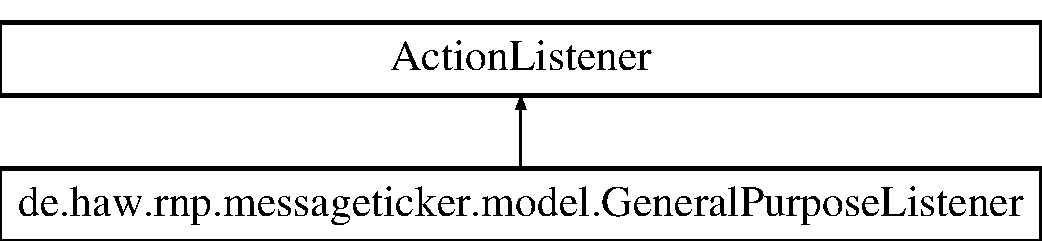
\includegraphics[height=2.000000cm]{classde_1_1haw_1_1rnp_1_1messageticker_1_1model_1_1GeneralPurposeListener}
\end{center}
\end{figure}
\subsection*{Public Member Functions}
\begin{DoxyCompactItemize}
\item 
\hypertarget{classde_1_1haw_1_1rnp_1_1messageticker_1_1model_1_1GeneralPurposeListener_afb387410079c4b47f9fcbb301da7e972}{{\bfseries General\-Purpose\-Listener} (\hyperlink{classde_1_1haw_1_1rnp_1_1messageticker_1_1Controller}{Controller} controller)}\label{classde_1_1haw_1_1rnp_1_1messageticker_1_1model_1_1GeneralPurposeListener_afb387410079c4b47f9fcbb301da7e972}

\item 
\hypertarget{classde_1_1haw_1_1rnp_1_1messageticker_1_1model_1_1GeneralPurposeListener_a70a06b0de2550eab21afd2637e4beaeb}{void {\bfseries action\-Performed} (Action\-Event e)}\label{classde_1_1haw_1_1rnp_1_1messageticker_1_1model_1_1GeneralPurposeListener_a70a06b0de2550eab21afd2637e4beaeb}

\end{DoxyCompactItemize}


\subsection{Detailed Description}
Listener that just forwards the actions back to the controller (for better modularity). 

The documentation for this class was generated from the following file\-:\begin{DoxyCompactItemize}
\item 
src/main/java/de/haw/rnp/messageticker/model/General\-Purpose\-Listener.\-java\end{DoxyCompactItemize}

\hypertarget{classde_1_1haw_1_1rnp_1_1messageticker_1_1Main}{\section{de.\-haw.\-rnp.\-messageticker.\-Main Class Reference}
\label{classde_1_1haw_1_1rnp_1_1messageticker_1_1Main}\index{de.\-haw.\-rnp.\-messageticker.\-Main@{de.\-haw.\-rnp.\-messageticker.\-Main}}
}
\subsection*{Static Public Member Functions}
\begin{DoxyCompactItemize}
\item 
\hypertarget{classde_1_1haw_1_1rnp_1_1messageticker_1_1Main_a26be98cd60a111da6895a2f842f48812}{static void {\bfseries main} (String\mbox{[}$\,$\mbox{]} args)}\label{classde_1_1haw_1_1rnp_1_1messageticker_1_1Main_a26be98cd60a111da6895a2f842f48812}

\end{DoxyCompactItemize}


The documentation for this class was generated from the following file\-:\begin{DoxyCompactItemize}
\item 
src/main/java/de/haw/rnp/messageticker/Main.\-java\end{DoxyCompactItemize}

\hypertarget{classde_1_1haw_1_1rnp_1_1messageticker_1_1model_1_1Message}{\section{de.\-haw.\-rnp.\-messageticker.\-model.\-Message Class Reference}
\label{classde_1_1haw_1_1rnp_1_1messageticker_1_1model_1_1Message}\index{de.\-haw.\-rnp.\-messageticker.\-model.\-Message@{de.\-haw.\-rnp.\-messageticker.\-model.\-Message}}
}


This class represents a message.  


\subsection*{Public Member Functions}
\begin{DoxyCompactItemize}
\item 
\hyperlink{classde_1_1haw_1_1rnp_1_1messageticker_1_1model_1_1Message_ac95495a6f00dbda08ab5ee772886f1bd}{Message} (String type, String content)
\begin{DoxyCompactList}\small\item\em Constructs a new content model. \end{DoxyCompactList}\item 
\hypertarget{classde_1_1haw_1_1rnp_1_1messageticker_1_1model_1_1Message_ac762c97b4f90cb2b4e4f7d35b88ac46b}{String {\bfseries get\-Type} ()}\label{classde_1_1haw_1_1rnp_1_1messageticker_1_1model_1_1Message_ac762c97b4f90cb2b4e4f7d35b88ac46b}

\item 
\hypertarget{classde_1_1haw_1_1rnp_1_1messageticker_1_1model_1_1Message_aa5296edf418ad44a2d064b424dcc9d1a}{void {\bfseries set\-Type} (String type)}\label{classde_1_1haw_1_1rnp_1_1messageticker_1_1model_1_1Message_aa5296edf418ad44a2d064b424dcc9d1a}

\item 
\hypertarget{classde_1_1haw_1_1rnp_1_1messageticker_1_1model_1_1Message_a9601ba408710f1b7d1f3e7b1ac8b9697}{String {\bfseries get\-Content} ()}\label{classde_1_1haw_1_1rnp_1_1messageticker_1_1model_1_1Message_a9601ba408710f1b7d1f3e7b1ac8b9697}

\item 
\hypertarget{classde_1_1haw_1_1rnp_1_1messageticker_1_1model_1_1Message_addf2895714909698f20fd7520c19b4f1}{void {\bfseries set\-Content} (String content)}\label{classde_1_1haw_1_1rnp_1_1messageticker_1_1model_1_1Message_addf2895714909698f20fd7520c19b4f1}

\item 
\hypertarget{classde_1_1haw_1_1rnp_1_1messageticker_1_1model_1_1Message_aa65c5da2412a4fd68c8f852fd1667da1}{String {\bfseries to\-String} ()}\label{classde_1_1haw_1_1rnp_1_1messageticker_1_1model_1_1Message_aa65c5da2412a4fd68c8f852fd1667da1}

\end{DoxyCompactItemize}


\subsection{Detailed Description}
This class represents a message. 

Every message has a content and a type. 

\subsection{Constructor \& Destructor Documentation}
\hypertarget{classde_1_1haw_1_1rnp_1_1messageticker_1_1model_1_1Message_ac95495a6f00dbda08ab5ee772886f1bd}{\index{de\-::haw\-::rnp\-::messageticker\-::model\-::\-Message@{de\-::haw\-::rnp\-::messageticker\-::model\-::\-Message}!Message@{Message}}
\index{Message@{Message}!de::haw::rnp::messageticker::model::Message@{de\-::haw\-::rnp\-::messageticker\-::model\-::\-Message}}
\subsubsection[{Message}]{\setlength{\rightskip}{0pt plus 5cm}de.\-haw.\-rnp.\-messageticker.\-model.\-Message.\-Message (
\begin{DoxyParamCaption}
\item[{String}]{type, }
\item[{String}]{content}
\end{DoxyParamCaption}
)}}\label{classde_1_1haw_1_1rnp_1_1messageticker_1_1model_1_1Message_ac95495a6f00dbda08ab5ee772886f1bd}


Constructs a new content model. 


\begin{DoxyParams}{Parameters}
{\em type} & the type of the news as String \\
\hline
{\em content} & actual content of the news \\
\hline
\end{DoxyParams}


The documentation for this class was generated from the following file\-:\begin{DoxyCompactItemize}
\item 
src/main/java/de/haw/rnp/messageticker/model/Message.\-java\end{DoxyCompactItemize}

\hypertarget{classde_1_1haw_1_1rnp_1_1messageticker_1_1model_1_1MessageProducer}{\section{de.\-haw.\-rnp.\-messageticker.\-model.\-Message\-Producer Class Reference}
\label{classde_1_1haw_1_1rnp_1_1messageticker_1_1model_1_1MessageProducer}\index{de.\-haw.\-rnp.\-messageticker.\-model.\-Message\-Producer@{de.\-haw.\-rnp.\-messageticker.\-model.\-Message\-Producer}}
}


Producer in the consumer producer pattern.  


Inheritance diagram for de.\-haw.\-rnp.\-messageticker.\-model.\-Message\-Producer\-:\begin{figure}[H]
\begin{center}
\leavevmode
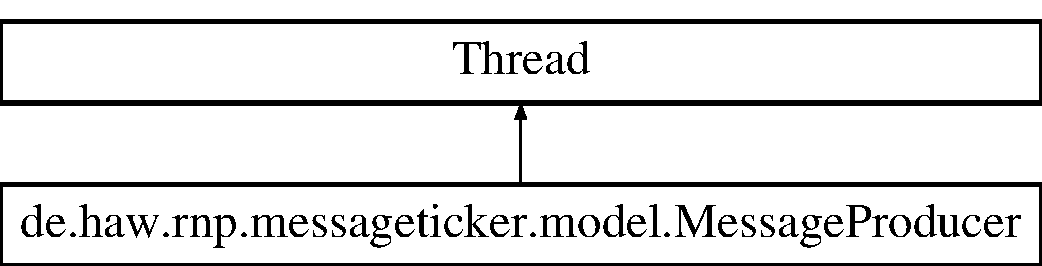
\includegraphics[height=2.000000cm]{classde_1_1haw_1_1rnp_1_1messageticker_1_1model_1_1MessageProducer}
\end{center}
\end{figure}
\subsection*{Public Member Functions}
\begin{DoxyCompactItemize}
\item 
\hyperlink{classde_1_1haw_1_1rnp_1_1messageticker_1_1model_1_1MessageProducer_a87904a84507bffe8983f275cd15b8f81}{Message\-Producer} (Linked\-Blocking\-Queue shared\-Memory)
\begin{DoxyCompactList}\small\item\em Constructs the producer. \end{DoxyCompactList}\item 
\hypertarget{classde_1_1haw_1_1rnp_1_1messageticker_1_1model_1_1MessageProducer_ae3e7a64de567365dfde2882a2b9e96aa}{void \hyperlink{classde_1_1haw_1_1rnp_1_1messageticker_1_1model_1_1MessageProducer_ae3e7a64de567365dfde2882a2b9e96aa}{run} ()}\label{classde_1_1haw_1_1rnp_1_1messageticker_1_1model_1_1MessageProducer_ae3e7a64de567365dfde2882a2b9e96aa}

\begin{DoxyCompactList}\small\item\em Uses the \hyperlink{classde_1_1haw_1_1rnp_1_1messageticker_1_1model_1_1RandomGenerator}{Random\-Generator} to produce random messages at random intervals (1s-\/5s). \end{DoxyCompactList}\end{DoxyCompactItemize}


\subsection{Detailed Description}
Producer in the consumer producer pattern. 

Produces random messages. 

\subsection{Constructor \& Destructor Documentation}
\hypertarget{classde_1_1haw_1_1rnp_1_1messageticker_1_1model_1_1MessageProducer_a87904a84507bffe8983f275cd15b8f81}{\index{de\-::haw\-::rnp\-::messageticker\-::model\-::\-Message\-Producer@{de\-::haw\-::rnp\-::messageticker\-::model\-::\-Message\-Producer}!Message\-Producer@{Message\-Producer}}
\index{Message\-Producer@{Message\-Producer}!de::haw::rnp::messageticker::model::MessageProducer@{de\-::haw\-::rnp\-::messageticker\-::model\-::\-Message\-Producer}}
\subsubsection[{Message\-Producer}]{\setlength{\rightskip}{0pt plus 5cm}de.\-haw.\-rnp.\-messageticker.\-model.\-Message\-Producer.\-Message\-Producer (
\begin{DoxyParamCaption}
\item[{Linked\-Blocking\-Queue}]{shared\-Memory}
\end{DoxyParamCaption}
)}}\label{classde_1_1haw_1_1rnp_1_1messageticker_1_1model_1_1MessageProducer_a87904a84507bffe8983f275cd15b8f81}


Constructs the producer. 


\begin{DoxyParams}{Parameters}
{\em shared\-Memory} & Shared memory (buffer) for the produced items. \\
\hline
\end{DoxyParams}


The documentation for this class was generated from the following file\-:\begin{DoxyCompactItemize}
\item 
src/main/java/de/haw/rnp/messageticker/model/Message\-Producer.\-java\end{DoxyCompactItemize}

\hypertarget{classde_1_1haw_1_1rnp_1_1messageticker_1_1view_1_1MessagesView}{\section{de.\-haw.\-rnp.\-messageticker.\-view.\-Messages\-View Class Reference}
\label{classde_1_1haw_1_1rnp_1_1messageticker_1_1view_1_1MessagesView}\index{de.\-haw.\-rnp.\-messageticker.\-view.\-Messages\-View@{de.\-haw.\-rnp.\-messageticker.\-view.\-Messages\-View}}
}


The view for displaying all messages and the basic chat functionality.  


Inheritance diagram for de.\-haw.\-rnp.\-messageticker.\-view.\-Messages\-View\-:\begin{figure}[H]
\begin{center}
\leavevmode
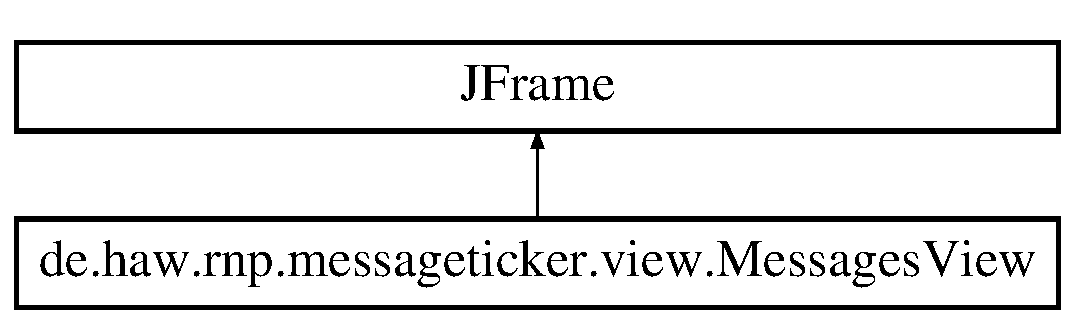
\includegraphics[height=2.000000cm]{classde_1_1haw_1_1rnp_1_1messageticker_1_1view_1_1MessagesView}
\end{center}
\end{figure}
\subsection*{Public Member Functions}
\begin{DoxyCompactItemize}
\item 
\hyperlink{classde_1_1haw_1_1rnp_1_1messageticker_1_1view_1_1MessagesView_ace78674474b3d8b311d8fc71d19a7ea1}{Messages\-View} (String\mbox{[}$\,$\mbox{]} message\-Types)
\begin{DoxyCompactList}\small\item\em Constructs the view. \end{DoxyCompactList}\item 
\hypertarget{classde_1_1haw_1_1rnp_1_1messageticker_1_1view_1_1MessagesView_ab3d85c91f7caee763a846f92667f7c54}{void {\bfseries add\-Message} (\hyperlink{classde_1_1haw_1_1rnp_1_1messageticker_1_1model_1_1Message}{Message} message)}\label{classde_1_1haw_1_1rnp_1_1messageticker_1_1view_1_1MessagesView_ab3d85c91f7caee763a846f92667f7c54}

\item 
\hypertarget{classde_1_1haw_1_1rnp_1_1messageticker_1_1view_1_1MessagesView_af09195f64de6fd81efb6f841d488b3e3}{String {\bfseries get\-Message\-Input} ()}\label{classde_1_1haw_1_1rnp_1_1messageticker_1_1view_1_1MessagesView_af09195f64de6fd81efb6f841d488b3e3}

\item 
\hypertarget{classde_1_1haw_1_1rnp_1_1messageticker_1_1view_1_1MessagesView_ae8fe70097e29bd55b47a8a946e34be38}{J\-Button {\bfseries get\-Send} ()}\label{classde_1_1haw_1_1rnp_1_1messageticker_1_1view_1_1MessagesView_ae8fe70097e29bd55b47a8a946e34be38}

\item 
\hypertarget{classde_1_1haw_1_1rnp_1_1messageticker_1_1view_1_1MessagesView_adb1d205950cc3032f1af99d70d6a1b61}{J\-Button {\bfseries get\-Pause\-Threads} ()}\label{classde_1_1haw_1_1rnp_1_1messageticker_1_1view_1_1MessagesView_adb1d205950cc3032f1af99d70d6a1b61}

\item 
\hypertarget{classde_1_1haw_1_1rnp_1_1messageticker_1_1view_1_1MessagesView_a5e416aed4b29dcf5fd61285c1ca64a43}{J\-Label {\bfseries get\-Status\-Label} ()}\label{classde_1_1haw_1_1rnp_1_1messageticker_1_1view_1_1MessagesView_a5e416aed4b29dcf5fd61285c1ca64a43}

\item 
\hypertarget{classde_1_1haw_1_1rnp_1_1messageticker_1_1view_1_1MessagesView_a91e78461c65af32847d55e6b6be573f7}{String {\bfseries get\-Message\-Types\-Selector} ()}\label{classde_1_1haw_1_1rnp_1_1messageticker_1_1view_1_1MessagesView_a91e78461c65af32847d55e6b6be573f7}

\item 
\hypertarget{classde_1_1haw_1_1rnp_1_1messageticker_1_1view_1_1MessagesView_a96a5df46c197df4c2c8dfee577c123e3}{void {\bfseries register\-Send\-Button\-Listener} (Action\-Listener l)}\label{classde_1_1haw_1_1rnp_1_1messageticker_1_1view_1_1MessagesView_a96a5df46c197df4c2c8dfee577c123e3}

\item 
\hypertarget{classde_1_1haw_1_1rnp_1_1messageticker_1_1view_1_1MessagesView_a3306fcfebd2a947a9d5927b43e565e99}{void {\bfseries register\-Thread\-Button\-Listener} (Action\-Listener l)}\label{classde_1_1haw_1_1rnp_1_1messageticker_1_1view_1_1MessagesView_a3306fcfebd2a947a9d5927b43e565e99}

\end{DoxyCompactItemize}


\subsection{Detailed Description}
The view for displaying all messages and the basic chat functionality. 

\subsection{Constructor \& Destructor Documentation}
\hypertarget{classde_1_1haw_1_1rnp_1_1messageticker_1_1view_1_1MessagesView_ace78674474b3d8b311d8fc71d19a7ea1}{\index{de\-::haw\-::rnp\-::messageticker\-::view\-::\-Messages\-View@{de\-::haw\-::rnp\-::messageticker\-::view\-::\-Messages\-View}!Messages\-View@{Messages\-View}}
\index{Messages\-View@{Messages\-View}!de::haw::rnp::messageticker::view::MessagesView@{de\-::haw\-::rnp\-::messageticker\-::view\-::\-Messages\-View}}
\subsubsection[{Messages\-View}]{\setlength{\rightskip}{0pt plus 5cm}de.\-haw.\-rnp.\-messageticker.\-view.\-Messages\-View.\-Messages\-View (
\begin{DoxyParamCaption}
\item[{String\mbox{[}$\,$\mbox{]}}]{message\-Types}
\end{DoxyParamCaption}
)}}\label{classde_1_1haw_1_1rnp_1_1messageticker_1_1view_1_1MessagesView_ace78674474b3d8b311d8fc71d19a7ea1}


Constructs the view. 


\begin{DoxyParams}{Parameters}
{\em message\-Types} & establishes the message\-Types \\
\hline
\end{DoxyParams}


The documentation for this class was generated from the following file\-:\begin{DoxyCompactItemize}
\item 
src/main/java/de/haw/rnp/messageticker/view/Messages\-View.\-java\end{DoxyCompactItemize}

\hypertarget{classde_1_1haw_1_1rnp_1_1messageticker_1_1model_1_1MessageTest}{\section{de.\-haw.\-rnp.\-messageticker.\-model.\-Message\-Test Class Reference}
\label{classde_1_1haw_1_1rnp_1_1messageticker_1_1model_1_1MessageTest}\index{de.\-haw.\-rnp.\-messageticker.\-model.\-Message\-Test@{de.\-haw.\-rnp.\-messageticker.\-model.\-Message\-Test}}
}


Tests for the \hyperlink{classde_1_1haw_1_1rnp_1_1messageticker_1_1model_1_1Message}{Message} Model.  


\subsection*{Public Member Functions}
\begin{DoxyCompactItemize}
\item 
\hypertarget{classde_1_1haw_1_1rnp_1_1messageticker_1_1model_1_1MessageTest_afbfebc1651b9d9424418bd99a3813ed7}{void {\bfseries setup} ()}\label{classde_1_1haw_1_1rnp_1_1messageticker_1_1model_1_1MessageTest_afbfebc1651b9d9424418bd99a3813ed7}

\item 
\hypertarget{classde_1_1haw_1_1rnp_1_1messageticker_1_1model_1_1MessageTest_a80a0215d5c382d4a57eace0460e211a3}{void {\bfseries get\-Type} ()  throws Exception }\label{classde_1_1haw_1_1rnp_1_1messageticker_1_1model_1_1MessageTest_a80a0215d5c382d4a57eace0460e211a3}

\item 
\hypertarget{classde_1_1haw_1_1rnp_1_1messageticker_1_1model_1_1MessageTest_aad9efd82225ac06bba689cd3c278cb00}{void {\bfseries set\-Type} ()  throws Exception }\label{classde_1_1haw_1_1rnp_1_1messageticker_1_1model_1_1MessageTest_aad9efd82225ac06bba689cd3c278cb00}

\item 
\hypertarget{classde_1_1haw_1_1rnp_1_1messageticker_1_1model_1_1MessageTest_aa11eb10c39f456c34905d442ee6bf0fc}{void {\bfseries get\-Content} ()  throws Exception }\label{classde_1_1haw_1_1rnp_1_1messageticker_1_1model_1_1MessageTest_aa11eb10c39f456c34905d442ee6bf0fc}

\item 
\hypertarget{classde_1_1haw_1_1rnp_1_1messageticker_1_1model_1_1MessageTest_ab6daed916113c20b3d4409a4fcba5779}{void {\bfseries set\-Content} ()  throws Exception }\label{classde_1_1haw_1_1rnp_1_1messageticker_1_1model_1_1MessageTest_ab6daed916113c20b3d4409a4fcba5779}

\item 
\hypertarget{classde_1_1haw_1_1rnp_1_1messageticker_1_1model_1_1MessageTest_a6bf4adea40ed3636568b765d8c573a0c}{void {\bfseries test\-To\-String} ()}\label{classde_1_1haw_1_1rnp_1_1messageticker_1_1model_1_1MessageTest_a6bf4adea40ed3636568b765d8c573a0c}

\end{DoxyCompactItemize}


\subsection{Detailed Description}
Tests for the \hyperlink{classde_1_1haw_1_1rnp_1_1messageticker_1_1model_1_1Message}{Message} Model. 

The documentation for this class was generated from the following file\-:\begin{DoxyCompactItemize}
\item 
src/test/java/de/haw/rnp/messageticker/model/Message\-Test.\-java\end{DoxyCompactItemize}

\hypertarget{classde_1_1haw_1_1rnp_1_1messageticker_1_1model_1_1RandomGenerator}{\section{de.\-haw.\-rnp.\-messageticker.\-model.\-Random\-Generator Class Reference}
\label{classde_1_1haw_1_1rnp_1_1messageticker_1_1model_1_1RandomGenerator}\index{de.\-haw.\-rnp.\-messageticker.\-model.\-Random\-Generator@{de.\-haw.\-rnp.\-messageticker.\-model.\-Random\-Generator}}
}


Generator for random messages and other stuff with the singleton pattern.  


\subsection*{Public Member Functions}
\begin{DoxyCompactItemize}
\item 
\hypertarget{classde_1_1haw_1_1rnp_1_1messageticker_1_1model_1_1RandomGenerator_a6ece77ab7f3ecc6a2bfd38fc1b805525}{\hyperlink{classde_1_1haw_1_1rnp_1_1messageticker_1_1model_1_1RandomGenerator_a6ece77ab7f3ecc6a2bfd38fc1b805525}{Random\-Generator} ()}\label{classde_1_1haw_1_1rnp_1_1messageticker_1_1model_1_1RandomGenerator_a6ece77ab7f3ecc6a2bfd38fc1b805525}

\begin{DoxyCompactList}\small\item\em Overwrites and cancels normal constructor. \end{DoxyCompactList}\item 
String \hyperlink{classde_1_1haw_1_1rnp_1_1messageticker_1_1model_1_1RandomGenerator_a5c94e12d07cab557d86dff666e53c73f}{generate\-Random\-Message\-Type} ()
\begin{DoxyCompactList}\small\item\em Random message type. \end{DoxyCompactList}\item 
long \hyperlink{classde_1_1haw_1_1rnp_1_1messageticker_1_1model_1_1RandomGenerator_a25d71afe0223c919e1c64ffa2312a253}{generate\-Random\-Sleep\-Time} (int min\-Sleep\-Time, int max\-Sleep\-Time)
\begin{DoxyCompactList}\small\item\em Random sleep time for the thread in milliseconds. \end{DoxyCompactList}\item 
String \hyperlink{classde_1_1haw_1_1rnp_1_1messageticker_1_1model_1_1RandomGenerator_a49aa630dbb38447457fc2b253bfdfafa}{generate\-Random\-Message} ()
\begin{DoxyCompactList}\small\item\em Random message. \end{DoxyCompactList}\end{DoxyCompactItemize}
\subsection*{Static Public Member Functions}
\begin{DoxyCompactItemize}
\item 
static synchronized \hyperlink{classde_1_1haw_1_1rnp_1_1messageticker_1_1model_1_1RandomGenerator}{Random\-Generator} \hyperlink{classde_1_1haw_1_1rnp_1_1messageticker_1_1model_1_1RandomGenerator_a72560b6ba012d5fb0183fc0e798df219}{get\-Instance} ()
\begin{DoxyCompactList}\small\item\em Returns the singleton. \end{DoxyCompactList}\end{DoxyCompactItemize}


\subsection{Detailed Description}
Generator for random messages and other stuff with the singleton pattern. 

\subsection{Member Function Documentation}
\hypertarget{classde_1_1haw_1_1rnp_1_1messageticker_1_1model_1_1RandomGenerator_a49aa630dbb38447457fc2b253bfdfafa}{\index{de\-::haw\-::rnp\-::messageticker\-::model\-::\-Random\-Generator@{de\-::haw\-::rnp\-::messageticker\-::model\-::\-Random\-Generator}!generate\-Random\-Message@{generate\-Random\-Message}}
\index{generate\-Random\-Message@{generate\-Random\-Message}!de::haw::rnp::messageticker::model::RandomGenerator@{de\-::haw\-::rnp\-::messageticker\-::model\-::\-Random\-Generator}}
\subsubsection[{generate\-Random\-Message}]{\setlength{\rightskip}{0pt plus 5cm}String de.\-haw.\-rnp.\-messageticker.\-model.\-Random\-Generator.\-generate\-Random\-Message (
\begin{DoxyParamCaption}
{}
\end{DoxyParamCaption}
)}}\label{classde_1_1haw_1_1rnp_1_1messageticker_1_1model_1_1RandomGenerator_a49aa630dbb38447457fc2b253bfdfafa}


Random message. 

\begin{DoxyReturn}{Returns}
message 
\end{DoxyReturn}
\hypertarget{classde_1_1haw_1_1rnp_1_1messageticker_1_1model_1_1RandomGenerator_a5c94e12d07cab557d86dff666e53c73f}{\index{de\-::haw\-::rnp\-::messageticker\-::model\-::\-Random\-Generator@{de\-::haw\-::rnp\-::messageticker\-::model\-::\-Random\-Generator}!generate\-Random\-Message\-Type@{generate\-Random\-Message\-Type}}
\index{generate\-Random\-Message\-Type@{generate\-Random\-Message\-Type}!de::haw::rnp::messageticker::model::RandomGenerator@{de\-::haw\-::rnp\-::messageticker\-::model\-::\-Random\-Generator}}
\subsubsection[{generate\-Random\-Message\-Type}]{\setlength{\rightskip}{0pt plus 5cm}String de.\-haw.\-rnp.\-messageticker.\-model.\-Random\-Generator.\-generate\-Random\-Message\-Type (
\begin{DoxyParamCaption}
{}
\end{DoxyParamCaption}
)}}\label{classde_1_1haw_1_1rnp_1_1messageticker_1_1model_1_1RandomGenerator_a5c94e12d07cab557d86dff666e53c73f}


Random message type. 

\begin{DoxyReturn}{Returns}
\{\char`\"{}\-I\-N\-F\-O\char`\"{}, \char`\"{}\-W\-A\-R\-N\char`\"{}, \char`\"{}\-C\-O\-R\-R\char`\"{}\} any of those 
\end{DoxyReturn}
\hypertarget{classde_1_1haw_1_1rnp_1_1messageticker_1_1model_1_1RandomGenerator_a25d71afe0223c919e1c64ffa2312a253}{\index{de\-::haw\-::rnp\-::messageticker\-::model\-::\-Random\-Generator@{de\-::haw\-::rnp\-::messageticker\-::model\-::\-Random\-Generator}!generate\-Random\-Sleep\-Time@{generate\-Random\-Sleep\-Time}}
\index{generate\-Random\-Sleep\-Time@{generate\-Random\-Sleep\-Time}!de::haw::rnp::messageticker::model::RandomGenerator@{de\-::haw\-::rnp\-::messageticker\-::model\-::\-Random\-Generator}}
\subsubsection[{generate\-Random\-Sleep\-Time}]{\setlength{\rightskip}{0pt plus 5cm}long de.\-haw.\-rnp.\-messageticker.\-model.\-Random\-Generator.\-generate\-Random\-Sleep\-Time (
\begin{DoxyParamCaption}
\item[{int}]{min\-Sleep\-Time, }
\item[{int}]{max\-Sleep\-Time}
\end{DoxyParamCaption}
)}}\label{classde_1_1haw_1_1rnp_1_1messageticker_1_1model_1_1RandomGenerator_a25d71afe0223c919e1c64ffa2312a253}


Random sleep time for the thread in milliseconds. 

\begin{DoxyReturn}{Returns}
sleep time from 1000 -\/ 5000 ms 
\end{DoxyReturn}
\hypertarget{classde_1_1haw_1_1rnp_1_1messageticker_1_1model_1_1RandomGenerator_a72560b6ba012d5fb0183fc0e798df219}{\index{de\-::haw\-::rnp\-::messageticker\-::model\-::\-Random\-Generator@{de\-::haw\-::rnp\-::messageticker\-::model\-::\-Random\-Generator}!get\-Instance@{get\-Instance}}
\index{get\-Instance@{get\-Instance}!de::haw::rnp::messageticker::model::RandomGenerator@{de\-::haw\-::rnp\-::messageticker\-::model\-::\-Random\-Generator}}
\subsubsection[{get\-Instance}]{\setlength{\rightskip}{0pt plus 5cm}static synchronized {\bf Random\-Generator} de.\-haw.\-rnp.\-messageticker.\-model.\-Random\-Generator.\-get\-Instance (
\begin{DoxyParamCaption}
{}
\end{DoxyParamCaption}
)\hspace{0.3cm}{\ttfamily [static]}}}\label{classde_1_1haw_1_1rnp_1_1messageticker_1_1model_1_1RandomGenerator_a72560b6ba012d5fb0183fc0e798df219}


Returns the singleton. 

\begin{DoxyReturn}{Returns}
\hyperlink{classde_1_1haw_1_1rnp_1_1messageticker_1_1model_1_1RandomGenerator}{Random\-Generator} singleton 
\end{DoxyReturn}


The documentation for this class was generated from the following file\-:\begin{DoxyCompactItemize}
\item 
src/main/java/de/haw/rnp/messageticker/model/Random\-Generator.\-java\end{DoxyCompactItemize}

\hypertarget{classde_1_1haw_1_1rnp_1_1messageticker_1_1model_1_1RandomGeneratorTest}{\section{de.\-haw.\-rnp.\-messageticker.\-model.\-Random\-Generator\-Test Class Reference}
\label{classde_1_1haw_1_1rnp_1_1messageticker_1_1model_1_1RandomGeneratorTest}\index{de.\-haw.\-rnp.\-messageticker.\-model.\-Random\-Generator\-Test@{de.\-haw.\-rnp.\-messageticker.\-model.\-Random\-Generator\-Test}}
}


Tests the \hyperlink{classde_1_1haw_1_1rnp_1_1messageticker_1_1model_1_1RandomGenerator}{Random\-Generator}.  


\subsection*{Public Member Functions}
\begin{DoxyCompactItemize}
\item 
\hypertarget{classde_1_1haw_1_1rnp_1_1messageticker_1_1model_1_1RandomGeneratorTest_a2c816510f48220b44ff7d6bb66e2cac7}{void {\bfseries test\-Get\-Instance} ()  throws Exception }\label{classde_1_1haw_1_1rnp_1_1messageticker_1_1model_1_1RandomGeneratorTest_a2c816510f48220b44ff7d6bb66e2cac7}

\item 
\hypertarget{classde_1_1haw_1_1rnp_1_1messageticker_1_1model_1_1RandomGeneratorTest_a16dd54feb1edc7ac408d0f0c49609fad}{void {\bfseries test\-Generate\-Random\-Message\-Type} ()  throws Exception }\label{classde_1_1haw_1_1rnp_1_1messageticker_1_1model_1_1RandomGeneratorTest_a16dd54feb1edc7ac408d0f0c49609fad}

\item 
\hypertarget{classde_1_1haw_1_1rnp_1_1messageticker_1_1model_1_1RandomGeneratorTest_aaa386fae73ac945f8700b1a590a2fef7}{void {\bfseries test\-Generate\-Random\-Sleep\-Time} ()  throws Exception }\label{classde_1_1haw_1_1rnp_1_1messageticker_1_1model_1_1RandomGeneratorTest_aaa386fae73ac945f8700b1a590a2fef7}

\item 
\hypertarget{classde_1_1haw_1_1rnp_1_1messageticker_1_1model_1_1RandomGeneratorTest_a809bb20e71f3475224f7c71e37495346}{void {\bfseries test\-Generate\-Random\-Message} ()  throws Exception }\label{classde_1_1haw_1_1rnp_1_1messageticker_1_1model_1_1RandomGeneratorTest_a809bb20e71f3475224f7c71e37495346}

\end{DoxyCompactItemize}


\subsection{Detailed Description}
Tests the \hyperlink{classde_1_1haw_1_1rnp_1_1messageticker_1_1model_1_1RandomGenerator}{Random\-Generator}. 

The documentation for this class was generated from the following file\-:\begin{DoxyCompactItemize}
\item 
src/test/java/de/haw/rnp/messageticker/model/Random\-Generator\-Test.\-java\end{DoxyCompactItemize}

%--- End generated contents ---

% Index
\newpage
\phantomsection
\addcontentsline{toc}{chapter}{Index}
\printindex

\end{document}
